\documentclass[14pt]{extarticle}
\usepackage[T1]{fontenc}
\usepackage[utf8]{inputenc}
\usepackage{amsthm,amsmath,amssymb,braket,graphicx,enumitem,booktabs,multirow,booktabs,tcolorbox,wrapfig,cancel,caption}
\usepackage[margin=1in, top=0.5in]{geometry}
\usepackage{charter}
\begin{document}
\title{Lax Pairs and Double Bracket Flows}
\author{}
\date{}
\maketitle
\section{Definition of a Lax Pair}
Two operator \(A\) and \(B\) are said to form a lax pair if they satisfy the equation
\begin{equation}\begin{aligned}
	\label{lax}
	\frac{\mathrm{d}A(t)}{\mathrm{d}t} = \left[B(t), A(t)\right]
\end{aligned}\end{equation}
\section{Unitary Nature of the Flow}
It can be shown that this defines a unitary time evolution on \(A(t)\), in the following manner. Let \(U(t,t_0)\) be the unitary operator that carries this evolution through. We then need to construct a \(U(t,t_0)\). 
\begin{equation}
	A(t) = U(t,t_0) A(t_0) U^\dagger (t,t_0)
\end{equation}
where \(A(t_0)\) is the operator \(A\) at a particular time \(t_0\). The time change of \(A\) can then be written as
\begin{equation}\begin{aligned}
	\frac{\mathrm{d}A(t)}{\mathrm{d}t} &= \frac{\mathrm{d}U(t, t_0)}{\mathrm{d}t} A(t_0) U^\dagger(t,t_0) + U(t,t_0) A(t_0) \frac{\mathrm{d}U^\dagger(t, t_0)}{\mathrm{d}t}\\
					   &= \frac{\mathrm{d}U(t, t_0)}{\mathrm{d}t} U^\dagger(t,t_0) A(t) + A(t) U(t,t_0) \frac{\mathrm{d}U^\dagger(t, t_0)}{\mathrm{d}t} && \left[ A(t) = U A U^\dagger\right]\\ 
					   &= \frac{\mathrm{d}U(t, t_0)}{\mathrm{d}t} U^\dagger(t,t_0) A(t) - A(t) \frac{\mathrm{d}U(t, t_0)}{\mathrm{d}t} U^\dagger(t,t_0) && \left[ U U^\dagger = 1 \right]\\ 
					   &= \left[\frac{\mathrm{d}U(t, t_0)}{\mathrm{d}t} U^\dagger(t,t_0), A(t)\right]
\end{aligned}\end{equation}
Looking at the definition of a lax pair, we can now make the connection
\begin{equation}\begin{aligned}
	\label{unitary}
	B(t) = \frac{\mathrm{d}U(t, t_0)}{\mathrm{d}t} U^\dagger(t,t_0)
\end{aligned}\end{equation}

\textbf{The equation of motion characterised by the lax pair eq.~\ref{lax} can thus be said to generate a family of unitarily connected operators \(A(t)\), related by the unitaries defined by eq.~\ref{unitary}. A direct corrolary is that the spectrum of \(A(t)\) is preserved during this evolution.}
\section{Double Bracket Flow}
The double bracket flows correspond to a special choice of the operator \(B(t)\): \(B(t) \equiv \left[A(t), C\right]\). A consequence of this choice is that the lax pair evolution then serves to minimize the commutator \(\left[A(t), C\right]\). To see how, we first write down a function
\begin{equation}
	\chi \equiv \text{Tr}\left(\left[A(t) - C\right]^2\right) = \text{Tr}\left[A(t)^2 + C^2 - A(t) C - C A(t)\right]
\end{equation}
Since \(A^2(t) = U A^2 U^\dagger\), we get \(\text{Tr}(A^2(t)) = \text{Tr}(A)\). Also, from the cyclic nature of trace, we can write \(\text{Tr}(A(t)C)=\text{Tr}(CA(t))\). These considerations (and the fact that \(C\) does not depend on \(t\)) allows us to write
\begin{equation}
	\frac{\mathrm{d} \chi}{\mathrm{d}t} = -2\text{Tr}\left(\frac{\mathrm{d} A(t)}{\mathrm{d}t}\;C\right) = -2\text{Tr}\left(\left[B(t),A(t)\right] C\right)
\end{equation}
Using the cyclic property of trace, this becomes
\begin{equation}\begin{aligned}
	\text{Tr}\left(\left[B(t),A(t)\right] C\right) &= \text{Tr}\left(B(t)A(t) C - A(t) B(t)C\right)\\
						       &= \text{Tr}\left(B(t)A(t) C - B(t)A(t) C\right)\\
						       &= \text{Tr}\left(B(t)\left[A(t), C\right]\right)\\
\end{aligned}\end{equation}
If we now substitute the choice of \(B(t)\) we made above, we get
\begin{equation}
	\frac{\mathrm{d} \chi}{\mathrm{d}t} = -2\text{Tr}\left(\left[A(t), C\right]^2\right) = -2\text{Tr}\left(B(t)^2\right) \leq 0
\end{equation}
Since \(\chi\), the way it is defined, must necessarily be positive semi-definite for all \(t\), it has a global minimum at \(\chi = 0\). Since the derivative \(\frac{\mathrm{d} \chi}{\mathrm{d}t}\) is always negative, it will take \(\chi\) towards its minimum. At the minimum, the time derivative must vanish, otherwise \(\chi(t)\) will become negative. This gives the result
\begin{equation}
	\lim_{t\to \infty}\frac{\mathrm{d} \chi}{\mathrm{d}t} = -2 \lim_{t\to \infty}\text{Tr}\left(\left[A(t), C\right]^2\right) = 0 \implies \lim_{t\to \infty}\left[A(t), C\right] = 0
\end{equation}
In other words, \textbf{the lax pair evolution of \(A(t)\) against \(\left[A(t),C\right]\) leads to the diagonalization of \(A(t)\) with respect to \(C\).} This can be used as an iterative algorithm to diagonalize a general matrix with respect to another matrix:
\begin{itemize}
	\item Define matrices A and B, A being the one we want to diagonalize w.r.t B
	\item Iteratively run the next two steps until a desired accuracy is reached
	\item Compute a new matrix C = A*B - B*A
	\item Change A as follows: A = A + C*A - A*c
\end{itemize}
\begin{center}
	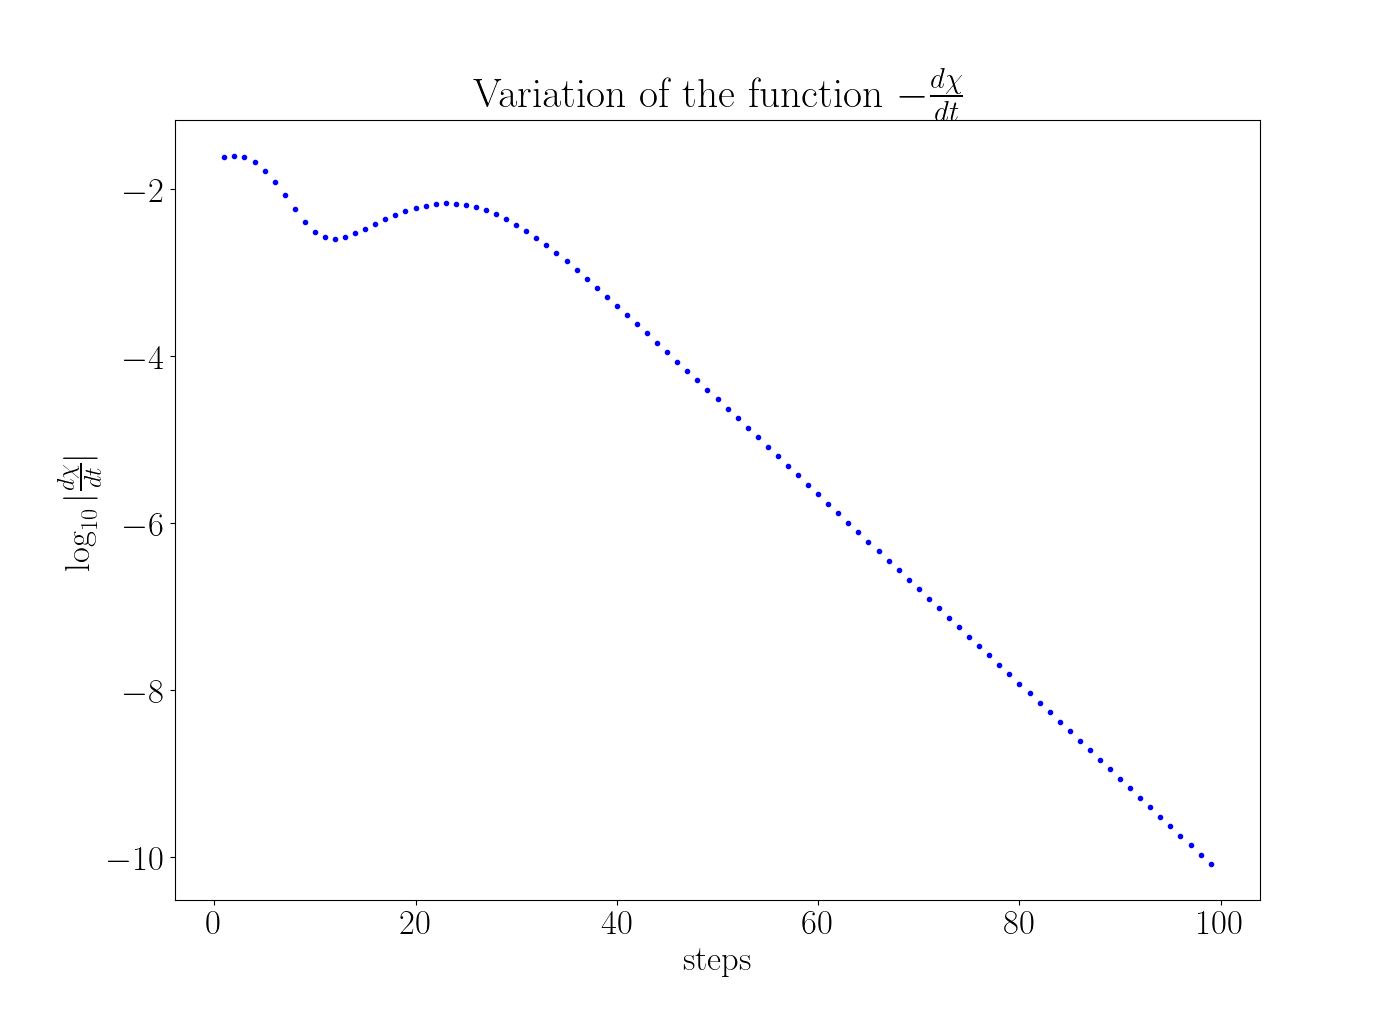
\includegraphics[scale=0.5]{Svsi.png}
	\captionof{figure}{Variation of the function \( \frac{\:\mathrm{d}\chi}{\:\mathrm{d}t}\) for an arbitrary choice of \(A\) and \(C\). The convergence of \(A\) towards a diagonal form is clear.}
\end{center}
The double bracket flow
\begin{equation}\begin{aligned}
	\frac{\:\mathrm{d}A}{\:\mathrm{d}t} = \left[  \left[ A, C \right], A  \right] 
\end{aligned}\end{equation}
is thus a flow towards the minima of the function \( \chi = \text{tr}\left( \left( A - C \right) ^2 \right)  \) .
\section{URG as a double-bracket flow}
The difference RG equation for URG can be written in the form
\begin{equation}
	\Delta \mathcal{H} (\omega,D) =  \frac{1}{\omega_1 - \omega_0}\left[G\left[ \mathcal{H}^d, \mathcal{H}^I\right],\mathcal{H}\right]\\
\end{equation}
This is not in the standard double-bracket form, primarily because it takes into account the off-diagonal terms in the Hamiltonian inside the generator of the unitary transformation. 
It can be given a double-bracket form by taking some approximations, as was shown in eq.~\ref{cuturg}.
\\\\
Just like the standard double-bracket flow equation, the URG equation acts as an optimizer - it minimizes the function
\begin{equation}
	\chi_j = \text{Tr}\left[\left(\mathcal{H}^I_j\right)^2\right]
\end{equation}
The definition of this function first requires a scheme to be defined. We can order the energy of the electrons as \(\epsilon_1 < \epsilon_2 < ... < \epsilon_j < ... < \epsilon_N\). The URG consists of sequentially decoupling the states \(\epsilon_N\), then \(\epsilon_{N-1}\), and so on. At the \(j^\text{th}\) step, the Hamiltonian can be partitioned in the subspace of the electron being decoupled; the partitioning looks like
\begin{equation}
	\mathcal{H}^0_j + c_j^\dagger T_j + T_j^\dagger c_j
\end{equation}
\(\mathcal{H}^0_j\) is the part that \textit{does not} scatter between \(\ket{\hat n_j} = 0,1\), while \(\mathcal{H}^I_j = c_j^\dagger T_j + T_j^\dagger c_j\) is the part that \textit{does} scatter between states with a definite value of \(\hat n_j\).
\\\\
The first observation that we make is that \(\chi_j\) is semi-positive definite. This is because it can be expressed as the norm-squared of a state vector.
\begin{equation}
	\chi_j = \sum_{i=1}^N \bra{\psi_i}\left(\mathcal{H}^I_j\right)^2\ket{\psi_i} = \sum_{i=1}^N \langle\phi_i | \phi_i \rangle \geq 0, \left[\text{where }\ket{\phi_i} = \mathcal{H}^I_j\ket{\psi_i}\right]
\end{equation}
The difference equation for \(\chi_j\) is
\begin{equation}\begin{aligned}
	\Delta \chi_j = 2\text{Tr}\left[\mathcal{H}^I_j\Delta \mathcal{H}^I_j\right] = 2\text{Tr}\left[\mathcal{H}^I_j\left(\mathcal{H}^I_{j-1} - \mathcal{H}^I_j\right)\right]\\
\end{aligned}\end{equation}
The first part of the trace is zero. To see why, note that from the nature of URG, once \(j\) has been decoupled, it is diagonal in all the subsequent Hamiltonians. Hence, \(\mathcal{H}_{j-1}^I\) will be diagonal in \(j\), while \(\mathcal{H}_j^I\) is, by definition, off-diagonal in \(j\). The product \(\mathcal{H}_j^I\mathcal{H}_{j-1}^I\) will hence be off-diagonal and will change \(\hat n_j\). Hence, it will vanish when taken inside a trace. What remains is
\begin{equation}\begin{aligned}
	\Delta \chi_j = -2\text{Tr}\left[\left(\mathcal{H}^I_j\right)^2\right] = -2 \chi_j\leq 0\\
\end{aligned}\end{equation}
At the fixed point \(j^*\) of URG, the off-diagonal part of the Hamiltonian vanishes, so we can write \(\mathcal{H}_{j^*}^I = 0 \implies \Delta \chi^* = 0\).
Combining the three points:
\begin{equation}\begin{aligned}
\chi_j \geq 0, && \Delta \chi_j \leq 0, && \Delta \chi_{j^*} = 0
\end{aligned}\end{equation}
we can say that URG starts from a non-minimal value of \(\chi\) and flows to its minimum \(\chi^* = 0\) at the fixed point.
\\\\
This minimization has been demonstrated numerically in fig.~\ref{minim}, where URG has been performed on a very simple model of potential scatter:\(\mathcal{H} = \sum_k \epsilon_k \hat n_k + J \sum_{k \neq k^\prime} c^\dagger_k c_{k^\prime}\).
\begin{center}
	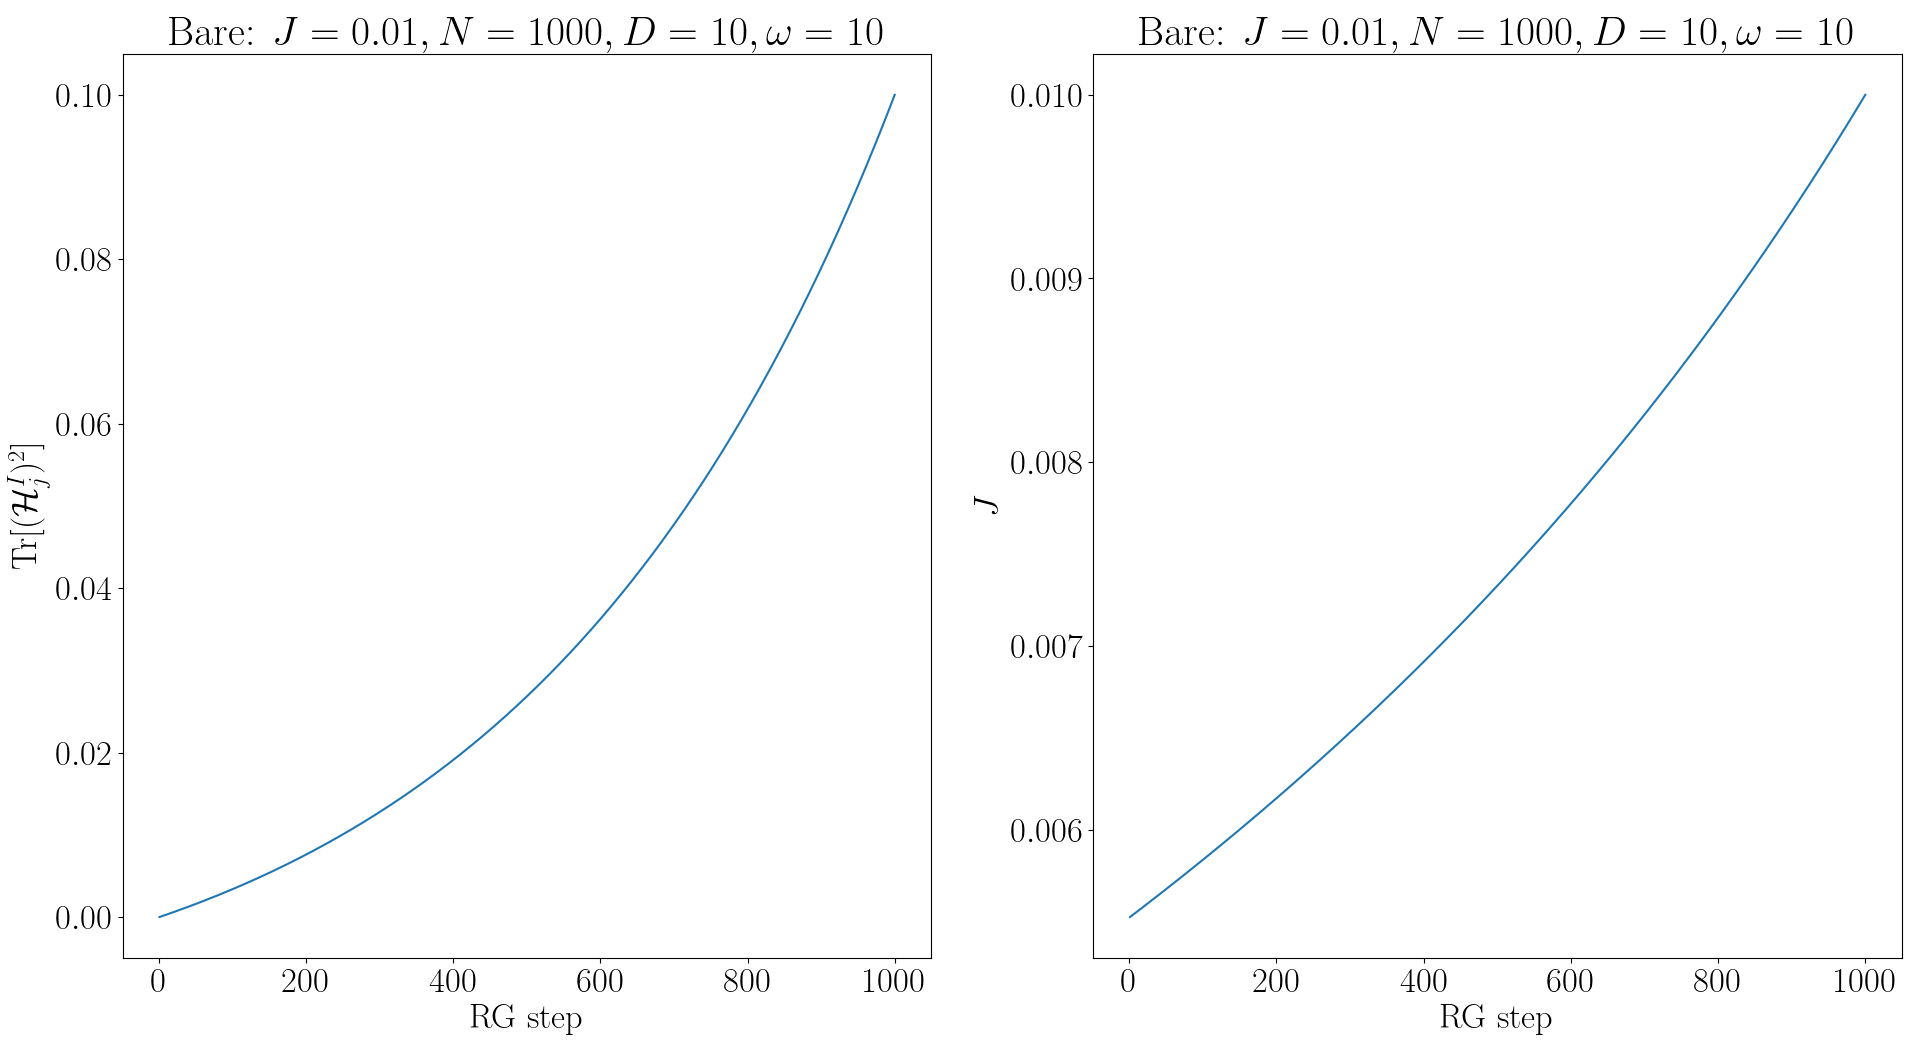
\includegraphics[scale=0.35]{decay1.png}
	\captionof{figure}{Variation of $J$ and $\chi$ for the potential scattering problem.}
	\label{minim}
\end{center}
\end{document}

